\documentclass{article}
\usepackage[svgnames]{xcolor}
\usepackage[utf8]{inputenc}
\usepackage{pdfpages}
\usepackage{float}
\usepackage{fullpage} % Package to use full page
\usepackage{parskip} % Package to tweak paragraph skipping
\usepackage{tikz} % Package for drawing
\usepackage{amsmath}
\usepackage{hyperref}
\hypersetup{
    colorlinks=true,
    linkcolor=purple,
    filecolor=magenta,      
    urlcolor=pink,
}
\usepackage{amssymb}
\usepackage{bm}
\usepackage{framed}
\usepackage{amsthm}
\usepackage{listings}
\usepackage{biblatex}

\lstset{language=R,
    basicstyle=\small\ttfamily,
    stringstyle=\color{DarkGreen},
    otherkeywords={0,1,2,3,4,5,6,7,8,9},
    morekeywords={TRUE,FALSE},
    deletekeywords={data,frame,length,as,character},
    keywordstyle=\color{blue},
    commentstyle=\color{DarkGreen},
}

\addbibresource{glm-exercises.bib}

\newenvironment{lyxcode}
	{\par\begin{list}{}{
		\setlength{\rightmargin}{\leftmargin}
		\setlength{\listparindent}{0pt}% needed for AMS classes
		\raggedright
		\setlength{\itemsep}{0pt}
		\setlength{\parsep}{0pt}
		\normalfont\ttfamily}%
	 \item[]}
	{\end{list}}


\newcommand\independent{\protect\mathpalette{\protect\independenT}{\perp}}
\def\independenT#1#2{\mathrel{\rlap{$#1#2$}\mkern2mu{#1#2}}}

\newcommand{\E}{\mathrm{E}}
\newcommand{\Var}{\mathrm{Var}}
\newcommand{\Cov}{\mathrm{Cov}}
\newcommand{\Cor}{\mathrm{Cor}}

% vertical line in {bmatrix}
\makeatletter
\renewcommand*\env@matrix[1][*\c@MaxMatrixCols c]{%
 \hskip -\arraycolsep
 \let\@ifnextchar\new@ifnextchar
 \array{#1}}
\makeatother

\title{Exercises in Generalized Linear Models \\ \textbf{Week 42}}
\author{Vinnie Ko, Jonas Moss, and Ørnulf Borgan}
\date{Fall 2020}

\begin{document}
\maketitle
Exercises for the course \href{https://www.uio.no/studier/emner/matnat/math/STK3100/}{STK3100/STK4100: Introduction to Generalized Linear Models} at the University of Oslo, fall 2020. The exercises are from the textbook Alan Agresti: \textit{Foundations of Linear and Generalized Linear Models}. Wiley, 2015. ISBN: 978-1-118-73003-4. The additional exercises are available \href{https://www.uio.no/studier/emner/matnat/math/STK3100/h20/oppgaver.html}{online}. Exercises exclusively nvolving \texttt{R} are not covered.
\section*{Additional Exercise 22}

\begin{lstlisting}
> # Enter the data
> lung.cancer.data = data.frame(
+   city = rep(1:4, each = 5),
+   age = rep(1:5, times = 4),
+   cases = c(11,11,11,10,11,13,6,15,10,12,4,8,7,11,9,5,7,10,14,8),
+   number = c(3059,800,710,581,509,2879,1083,923,834,634,3142,
+          1050,895,702,535,2520,878,839,631,539)
+   )
> lung.cancer.data[,"age"] = as.factor(lung.cancer.data[,"age"])
> lung.cancer.data[,"city"] = as.factor(lung.cancer.data[,"city"])
> head(lung.cancer.data)
  city age cases number
1    1   1    11   3059
2    1   2    11    800
3    1   3    11    710
4    1   4    10    581
5    1   5    11    509
6    2   1    13   2879
\end{lstlisting}


\subsection*{(a)}
The expected value of the response variable (\texttt{cases}) is proportional to the total number of male inhabitants (\texttt{number}). We here model the rate, i.e. $\frac{y_{i,j}}{n_{i,j}}$, where $y_{i,j}$ and $n_{i,j}$ are the number of cases and the number of inhabitants in city $i$ and age group $j$. The model $\E\left[\frac{Y_{i,j}}{n_{i,j}}\right] = e^{\eta_{i,j}}$ for a linear predictor $\eta_{i,j}$ hence corresponds to $\E\left[Y_{i,j}\right] = e^{\log n_{i,j} + \eta_{i,j}}$. So, we have to add $\log n_{i,j}$ as an offset to the linear predictor.


\vspace{\baselineskip}
\subsection*{(b)}

\begin{lstlisting}
> Poisson.model = glm(cases ~ offset(log(number)) + age + city, family = poisson, data = lung.cancer.data)
> summary(Poisson.model)

Call:
glm(formula = cases ~ offset(log(number)) + age + city, family = poisson, 
    data = lung.cancer.data)

Deviance Residuals: 
     Min        1Q    Median        3Q       Max  
-1.20728  -0.59302  -0.09784   0.58493   1.46574  

Coefficients:
            Estimate Std. Error z value Pr(>|z|)    
(Intercept)  -5.6455     0.2049 -27.555  < 2e-16 ***
age2          1.0961     0.2483   4.414 1.02e-05 ***
age3          1.5138     0.2317   6.534 6.39e-11 ***
age4          1.7584     0.2295   7.662 1.83e-14 ***
age5          1.8486     0.2354   7.855 4.01e-15 ***
city2        -0.1907     0.1910  -0.999   0.3180    
city3        -0.4791     0.2103  -2.279   0.0227 *  
city4        -0.2534     0.2033  -1.247   0.2125    
---

(Dispersion parameter for poisson family taken to be 1)

    Null deviance: 115.434  on 19  degrees of freedom
Residual deviance:  11.598  on 12  degrees of freedom
AIC: 109.07

Number of Fisher Scoring iterations: 4
\end{lstlisting}
The interpretation of $\widehat{\beta}$ can be done in the same way as in exercise 7.31 a) from the book.

\vspace{\baselineskip}
\subsection*{(c)}
\begin{lstlisting}
> lung.cancer.data[,"Fredericia"] = as.factor(as.numeric(lung.cancer.data[,"city"] == 1))
> head(lung.cancer.data)
  city age cases number Fredericia
1    1   1    11   3059          1
2    1   2    11    800          1
3    1   3    11    710          1
4    1   4    10    581          1
5    1   5    11    509          1
6    2   1    13   2879          0
> # Fit Poisson GLM
> Poisson.model.2 = glm(cases ~ offset(log(number)) + age + Fredericia, family = poisson, data = lung.cancer.data)
> summary(Poisson.model.2)

Call:
glm(formula = cases ~ offset(log(number)) + age + Fredericia, 
    family = poisson, data = lung.cancer.data)

Deviance Residuals: 
     Min        1Q    Median        3Q       Max  
-1.62564  -0.59506  -0.03471   0.17297   1.81669  

Coefficients:
            Estimate Std. Error z value Pr(>|z|)    
(Intercept)  -5.9502     0.1818 -32.736  < 2e-16 ***
age2          1.0997     0.2483   4.429 9.47e-06 ***
age3          1.5187     0.2316   6.556 5.51e-11 ***
age4          1.7671     0.2294   7.704 1.32e-14 ***
age5          1.8582     0.2352   7.899 2.82e-15 ***
Fredericia1   0.2991     0.1606   1.863   0.0624 .  
---

(Dispersion parameter for poisson family taken to be 1)

    Null deviance: 115.434  on 19  degrees of freedom
Residual deviance:  13.663  on 14  degrees of freedom
AIC: 107.14

Number of Fisher Scoring iterations: 4

> 
> # Likelihood ratio test.
> anova(Poisson.model.2, Poisson.model.1)
Analysis of Deviance Table

Model 1: cases ~ offset(log(number)) + age + Fredericia
Model 2: cases ~ offset(log(number)) + age + city
  Resid. Df Resid. Dev Df Deviance
1        14     13.663            
2        12     11.598  2   2.0658
> 1 - pchisq(anova(Poisson.model.2, Poisson.model.1)$Deviance[2], df = 1)
[1] 0.1506362
\end{lstlisting}

The two models are nested. So, we use the likelihood ratio test.\\
p = $0.1506 > 0.05$. So, we keep the null hypothesis and conclude that the model with simplified city effect is a better model.


\vspace{\baselineskip}
\subsection*{(d)}
Rate ratio of new lung cancer cases in Fredericia compared to the three other cities:
$\frac{\E\left[Y|x_{\mathrm{Fredericia}} = 1\right]}{\E\left[Y|x_{\mathrm{Fredericia}} = 0\right]} = \exp\left[\beta_{\mathrm{Fredericia}}\right]$.

\begin{lstlisting}
> # Estimated rate ratio
> exp(summary(Poisson.model.2)$coefficients["Fredericia1","Estimate"])
[1] 1.348685
> # 95% confidence interval of rate ratio
> exp(confint.default(Poisson.model.2))["Fredericia1",]
    2.5 %    97.5 % 
0.9845689 1.8474606 
\end{lstlisting}


\vspace{\baselineskip}
\subsection*{(e)}
\begin{lstlisting}
> # Numeric version of variable age
> lung.cancer.data[,"age.numeric"] = rep(
+   c(mean(40,55), mean(55,60), mean(60,65), mean(65,70), mean(70,75)),
+   times = 4
+   )
> # Fit Poisson GLM
> Poisson.model.3 = glm(cases ~ offset(log(number)) + I(age.numeric-40) + Fredericia, family = poisson, data = lung.cancer.data)
> summary(Poisson.model.3)

Call:
glm(formula = cases ~ offset(log(number)) + I(age.numeric - 40) + 
    Fredericia, family = poisson, data = lung.cancer.data)

Deviance Residuals: 
    Min       1Q   Median       3Q      Max  
-1.8683  -0.6997  -0.1695   0.3869   1.6274  

Coefficients:
                     Estimate Std. Error z value Pr(>|z|)    
(Intercept)         -5.857611   0.158061 -37.059   <2e-16 ***
I(age.numeric - 40)  0.064311   0.006945   9.261   <2e-16 ***
Fredericia1          0.290371   0.160441   1.810   0.0703 .  
---

(Dispersion parameter for poisson family taken to be 1)

    Null deviance: 115.434  on 19  degrees of freedom
Residual deviance:  16.141  on 17  degrees of freedom
AIC: 103.61

Number of Fisher Scoring iterations: 4

> 
> # Likelihood ratio test.
> anova(Poisson.model.3, Poisson.model.2)
Analysis of Deviance Table

Model 1: cases ~ offset(log(number)) + I(age.numeric - 40) + Fredericia
Model 2: cases ~ offset(log(number)) + age + Fredericia
  Resid. Df Resid. Dev Df Deviance
1        17     16.141            
2        14     13.663  3   2.4776
> 1 - pchisq(anova(Poisson.model.3, Poisson.model.2)$Deviance[2], df = 1)
[1] 0.1154789
\end{lstlisting}

The two models are nested. So, we use the likelihood ratio test.\\
p = $0.1155 > 0.05$. So, we keep the null hypothesis and conclude that the model with numerified age effect is a better model.

The interpretation of $\widehat{\beta}_{\mathrm{age~numeric}}$: log rate ratio of one unit increase in \texttt{age numeric}.
\section*{Additional Exercise 23}
\subsection*{(a)}
Law of total expectation:
\begin{align*}
\E\left[\E\left[Y|X\right]\right] &= \E\left[\int_{-\infty}^{\infty} yf(y|X)\, dy \right]\\
&= \int_{-\infty}^{\infty} \left(\int_{-\infty}^{\infty} yf(y|x)\, dy\right) f(x) \, dx\\
&= \int_{-\infty}^{\infty} \left(\int_{-\infty}^{\infty} y\frac{f(x,y)}{f(x)}f(x) \, dy\right)\, dx\\
&= \int_{-\infty}^{\infty} \left(\int_{-\infty}^{\infty} y f(x,y) \, dy\right)\, dx\\
&= \int_{-\infty}^{\infty} \left(\int_{-\infty}^{\infty} y f(x,y) \, dx\right)\, dy\\
&= \int_{-\infty}^{\infty} y\left(\int_{-\infty}^{\infty} f(x,y) \, dx\right)\, dy\\
&= \int_{-\infty}^{\infty} y \, f(y)\, dy\\
&= \E\left[Y\right]
\end{align*}

\textbf{Remark:} In the measure-theoretic definition of the conditional expectation, the law of total expectation is even more trivial: For then $Z$ is a variant of the conditional expectation, i.e.,
\[
Z=E(Y\mid X),\quad\textrm{almost everywhere}
\]
if and only if
\[
\int_{A}ZdP=\int_{A}YdP,\ldots A\in\sigma(X),
\]
where $\sigma(X)$ is the sigma-algebra of $X$-measurable sets. Since
$\Omega\in\sigma(X)$, $\int_{\Omega}E(Y\mid X)dP=\int_{\Omega}YdP=E(Y)$. See e.g. Billingsley's book \parencite[Chapter 34]{Billingsley1995-pp}.



\subsection*{(b)}
By definition, $\Var(Y\mid X)=E(Y^{2}\mid X)-E(Y\mid X)^{2}$, and the law of total variance can be proved directly.
\begin{align*}
\Var(Y) &= \E\left[Y^{2}\right] - \E\left[Y\right]^{2}\\
&= \E\left[\E\left[Y^{2}|X\right]\right] - \left(\E\left[\E\left[Y|X\right]\right]\right)^{2}\\
&= \E\left[\Var\left(Y|X\right) + \left(\E\left[Y|X\right]\right)^{2}\right] - \left(\E\left[\E\left[Y|X\right]\right]\right)^{2}\\
&= \E\left[\Var\left(Y|X\right)\right] + \E\left[\left(\E\left[Y|X\right]\right)^{2}\right] - \left(\E\left[\E\left[Y|X\right]\right]\right)^{2}\\
&= \E\left[\Var\left(Y|X\right)\right] + \Var\left(\E\left[Y|X\right]\right)
\end{align*}


\vspace{\baselineskip}
\section*{Additional Exercise 24}
\subsection*{(a)}
We already did this many times in earlier exercises.

\vspace{\baselineskip}
\subsection*{(b)}
\subsubsection*{(i)}
$\exp\left[\beta_{\mathrm{\texttt{badh}}}\right] = \frac{\E\left[Y|x_{\mathrm{\texttt{badh}}} = 1\right]}{\E\left[Y|x_{\mathrm{\texttt{badh}}} = 0\right]}$.\\

So, the estimate of rate ratio is
\begin{align*}
\exp\left[\widehat{\beta}_{\mathrm{\texttt{badh}}}\right] = \exp\left[1.1409\right] = 3.1296.
\end{align*}

$95\%$ confidence interval for this rate ratio is
\begin{align*}
&\left[\exp\left[\widehat{\beta}_{\mathrm{\texttt{badh}}} - z_{0.975} \cdot \mathrm{SE}(\widehat{\beta}_{\mathrm{\texttt{badh}}})\right],~\exp\left[\widehat{\beta}_{\mathrm{\texttt{badh}}} + z_{0.975} \cdot \mathrm{SE}(\widehat{\beta}_{\mathrm{\texttt{badh}}})\right] \right]\\
&= \left[\exp[1.1409 - 1.96 \cdot 0.0399], \exp[1.1409 + 1.96 \cdot 0.0399]\right]\\
&= \left[\exp[1.0628], \exp[1.2190]\right]\\
&= [2.8944, 3.3839]
\end{align*}

\subsubsection*{(ii)}
$\exp\left[10\beta_{\mathrm{\texttt{age}}}\right] = \frac{\E\left[Y|x_{\mathrm{\texttt{age}}} = 50\right]}{\E\left[Y|x_{\mathrm{\texttt{age}}} = 40\right]}$.\\

So, the estimate of rate ratio is
\begin{align*}
\exp\left[10\cdot\widehat{\beta}_{\mathrm{\texttt{age}}}\right] = \exp\left[0.0556\right] = 1.0571.
\end{align*}

$95\%$ confidence interval for this rate ratio is
\begin{align*}
&\left[\exp\left[10\cdot\widehat{\beta}_{\mathrm{\texttt{age}}} - 10\cdot z_{0.975} \cdot \mathrm{SE}(\widehat{\beta}_{\mathrm{\texttt{age}}})\right],~\exp\left[10\cdot\widehat{\beta}_{\mathrm{\texttt{age}}} + 10\cdot z_{0.975} \cdot \mathrm{SE}(\widehat{\beta}_{\mathrm{\texttt{age}}})\right] \right]\\
&= [\exp[0.0556 - 1.96 \cdot 0.0168], \exp[0.0556 + 1.96 \cdot 0.0168]]\\
&= \left[\exp[0.0227], \exp[0.0884]\right]\\
&= [1.0230, 1.0924]
\end{align*}

\subsubsection*{(iii)}
$\{\widehat{\mu}|\texttt{age} = 40, \texttt{badh} = 0\} = \exp\left[\widehat{\beta}_{0} + \widehat{\beta}_{\texttt{age}}\cdot40 + \widehat{\beta}_{\texttt{badh}}\cdot0\right] = \exp\left[0.5888 + 0.0056*40\right] = \exp\left[0.810971\right] = 2.2501$

The confidence interval of this rate ratio is equal to the confidence interval of $e^{\eta}$ where $\eta = \beta_{0} + \beta_{\texttt{age}}\cdot40$. We would then first find a confidence interval of $\eta$. This takes the form $\widehat{\eta} \pm z_{1-\frac{\alpha}{2}}\cdot \mathrm{SE}(\widehat{\eta})$, where $\mathrm{SE}(\widehat{\eta}) = \sqrt{\widehat{\Var}(\widehat{\beta}_{0}) + 40^{2}\widehat{\Var}(\widehat{\beta}_{\texttt{age}}) + 2\cdot40\cdot \widehat{\Cov}\left(\widehat{\beta}_{0}, \widehat{\beta}_{\texttt{age}}\right)}$. So, we would need $\Cov\left(\widehat{\beta}_{0}, \widehat{\beta}_{\texttt{age}}\right)$.


\vspace{\baselineskip}
\subsection*{(c)}

\subsubsection*{(i)}
We estimate parameters by solving quasi-likelihood equations instead of the likelihood equations. However, since $\phi$ will cancel, the estimates are the same as for the Poisson model.

\subsubsection*{(ii)}
We compute the Pearson statistic $X^{2} = \sum_{i=1}^{n} \frac{(y_{i} - \widehat{\mu}_{i})^{2}}{\widehat{\mu}_{i}}$ for the Poisson model, and estimate $\phi$ by $\widehat{\phi} = \frac{X^{2}}{n-p}$ where $p = 3$.


\section*{Exercise 7.2}
The pmf of Poisson distribution is $f(y) = \frac{\mu^{y}}{y!}e^{-\mu}$. The corresponding log-likelihood function is $L(\bm{y}) = \log\mu\sum_{i=1}^{n}y_{i} - n\mu -\sum_{i}^{n}\log y_{i}!$. The MLE of $\mu$ is then $\widehat{\mu} = \overline{y}$. Thus, the likelihood-ratio statistic is

\begin{align*}
-2\left(L_{0} - L_{1}\right) &= 2\left(
\log\widehat{\mu}_{1}\sum_{i=1}^{n}y_{i} - n\widehat{\mu}_{1} -\sum_{i}^{n}\log y_{i}!
-\log\mu_{0}\sum_{i=1}^{n}y_{i} +n\mu_{0} +\sum_{i}^{n}\log y_{i}!
\right)\\
&= 2\left(\log\frac{\widehat{\mu}_{1}}{\mu_{0}}\sum_{i=1}^{n}y_{i} +n\left(\widehat{\mu}_{1} -\mu_{0}\right)\right)\\
&= 2\left(n\overline{y}\log\frac{\widehat{\mu}_{1}}{\mu_{0}} +n\left(\widehat{\mu}_{1} -\mu_{0}\right)\right)\\
&= 2\left(n\overline{y}\log\frac{\overline{y}}{\mu_{0}} +n\left(\overline{y} -\mu_{0}\right)\right).
\end{align*}
The likelihood-ratio statistics follows chi-squared distribution with degrees of freedom $1$. So, a $100(1-\alpha)\%$ confidence interval is given as the set of $\mu_{0}$ that satisfy
\begin{align*}
2\left(n\overline{y}\log\frac{\overline{y}}{\mu_{0}} +n\left(\overline{y} -\mu_{0}\right)\right) < \chi_{1}^{2}(\alpha).
\end{align*}
(See problem 2 i) of the mandatory assignment.)
\section*{Exercise 7.3}
The score and information of Poisson distribution are
\begin{align*}
S(\mu) &= \frac{\partial L(\bm{y})}{\partial \mu} = \frac{1}{\mu}\sum_{i=1}^{n}y_{i} -n = n\left(\frac{\overline{y}}{\mu}-1\right)\\
H(\mu) &= \frac{\partial^{2} L(\bm{y})}{\partial \mu^{2}} = -\frac{n\overline{y}}{\mu^{2}}\\
\mathcal{J}(\mu) &= \E\left[-\frac{\partial^{2} L(\bm{Y})}{\partial \mu^{2}}\right] = \frac{n}{\mu^{2}}\E\left[\overline{Y}\right] = \frac{n}{\mu}.
\end{align*}

So, the score test statistic is
\begin{align*}
\frac{S(\mu_{0})}{\sqrt{\mathcal{J}(\mu_{0})}} = \frac{n\left(\frac{\overline{y}}{\mu_{0}}-1\right)}{\frac{n}{\mu_{0}}} = \frac{\sqrt{n}(\overline{y}-\mu_{0})}{\sqrt{\mu_{0}}} = \sim N(0,1).
\end{align*}

Thus, a $100(1-\alpha)\%$ confidence interval is given as the set of $\mu_{0}$ that satisfy
\begin{align*}
\left|\frac{\sqrt{n}(\overline{y}-\mu_{0})}{\sqrt{\mu_{0}}}\right| < z_{1-\frac{\alpha}{2}}.
\end{align*}
\section*{Exercise 7.4}
Let $Y_{1},Y_{2}$ be Poisson with parameters $\mu_{1}$ and $\mu_{2}$
and $H_{0}:\mu_{1}=\mu_{2}$. The likelihood-ratio statistic is
\begin{eqnarray*}
-2\log\left[\frac{\sup_{\mu}f(y_{1};\mu)f(y_{2};\mu)}{\sup_{\mu_{1},\mu_{2}}f(y_{1};\mu_{1})f(y_{2};\mu_{2})}\right] & = & -2\log\left[\frac{\sup_{\mu}\mu^{y_{1}+y_{2}}\frac{e^{-2\mu}}{y_{1}!y_{2}!}}{\sup_{\mu_{1}}\left(\mu_{1}^{y_{1}}\frac{e^{-\mu_{1}}}{y_{1}!}\right)\sup_{\mu_{2}}\left(\mu_{2}^{y_{2}}\frac{e^{-\mu_{2}}}{y_{2}!}\right)}\right].
\end{eqnarray*}
We already know that $\hat{\mu}_{1}=y_{1}$ and $\hat{\mu}_{2}=y_{2}$,
thus 
\[
\sup_{\mu_{1}}\left(\mu_{1}^{y_{1}}\frac{e^{-\mu_{1}}}{y_{1}!}\right)\sup_{\mu_{2}}\left(\mu_{2}^{y_{2}}\frac{e^{-\mu_{2}}}{y_{2}!}\right)=y_{1}^{y_{1}}\frac{e^{-y_{1}}}{y_{1}!}y_{2}^{y_{2}}\frac{e^{-y_{2}}}{y_{2}!}.
\]
On the other hand
\[
\log\left(\mu^{y_{1}+y_{2}}\frac{e^{-2\mu}}{y_{1}!y_{2}!}\right)=(y_{1}+y_{2})\log\mu-2\mu-\log(y_{1}!y_{2}!)
\]
Differentiate to find $\hat{\mu}=\frac{1}{2}(y_{1}+y_{2})$. The statistic
is
\[
-2\log\left[\frac{\left[\frac{1}{2}(y_{1}+y_{2})\right]^{y_{1}+y_{2}}\frac{e^{-(y_{1}+y_{2})}}{y_{1}!y_{2}!}}{y_{1}^{y_{1}}y_{2}^{y_{2}}\frac{e^{-y_{1}}}{y_{1}!}\frac{e^{-y_{2}}}{y_{2}!}}\right]=-2\log\left[\frac{\left[\frac{1}{2}(y_{1}+y_{2})\right]^{y_{1}+y_{2}}}{y_{1}^{y_{1}}y_{2}^{y_{2}}}\right]
\]
The asymptotic null distribution is $\chi^{2}(1)$. Since the sum
of Poissons is Poisson, the asymptotic approximation holds as $\mu\to\infty$. 

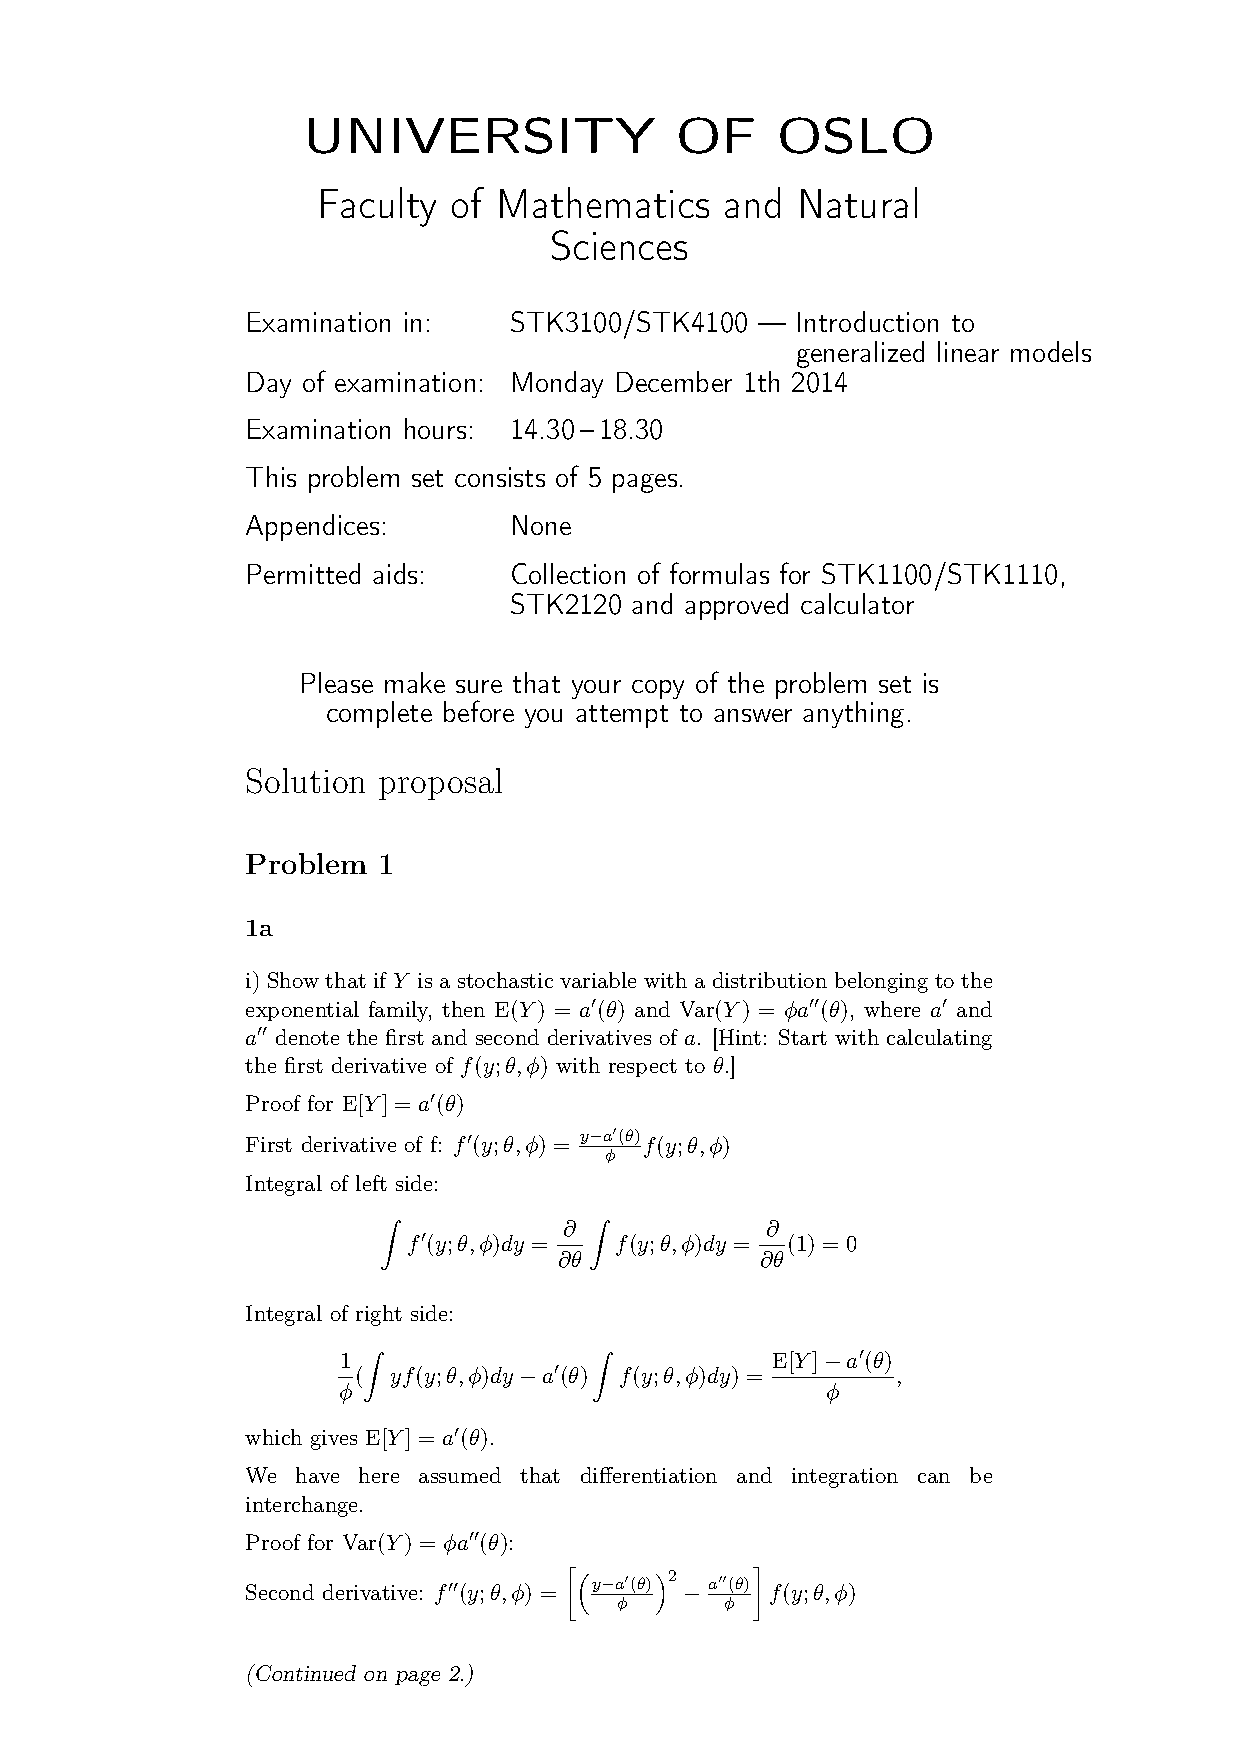
\includepdf[pages = {1,2,3}]{exam-exercises/exam-2014-solution.pdf}
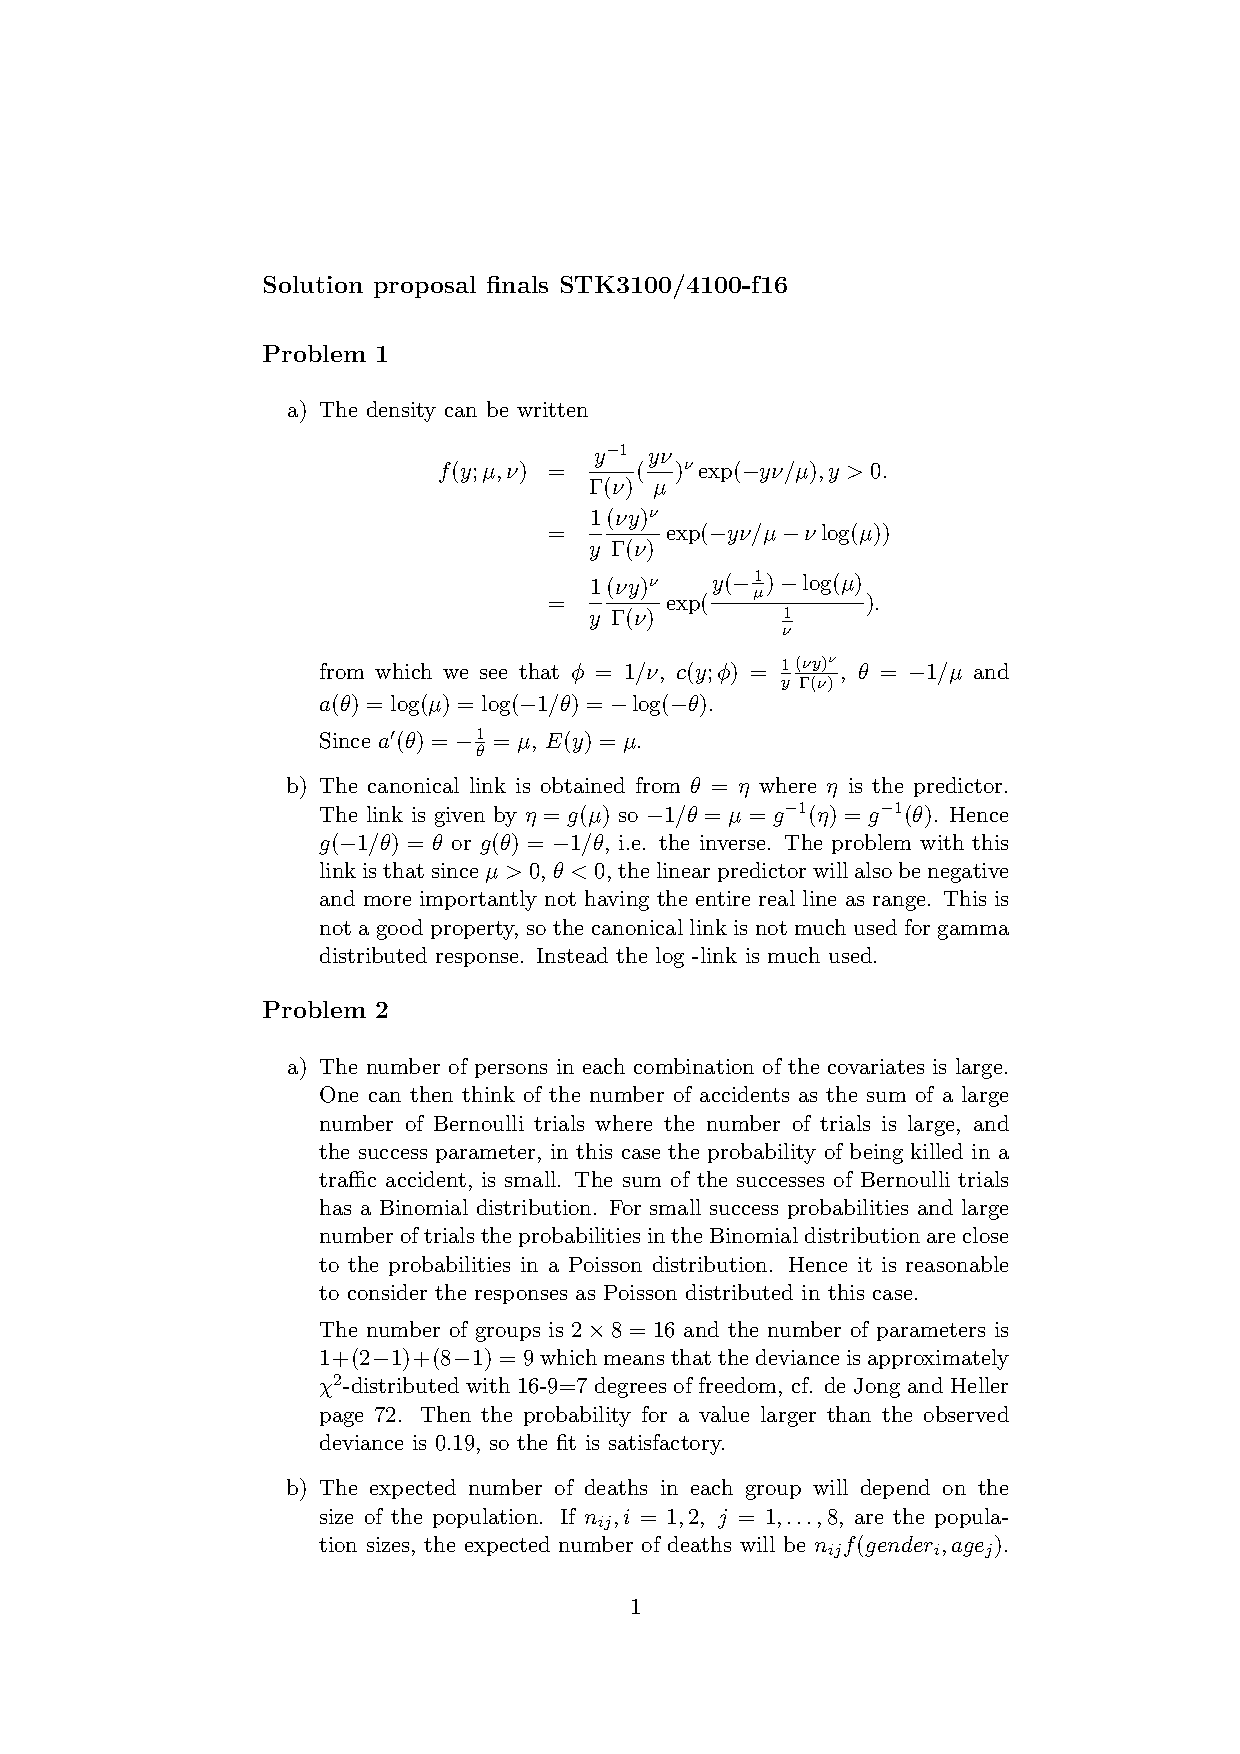
\includepdf[pages = {1,2,3}]{exam-exercises/exam-2016-solution.pdf}

\printbibliography
\end{document}
